\documentclass[sigconf,nonacm,10pt]{acmart}
\settopmatter{printacmref=false, printfolios=false}
\pagestyle{plain}
\usepackage{graphicx}
\usepackage{booktabs}
\usepackage{amsmath}
\usepackage{siunitx}
\graphicspath{{../figs/}}
\emergencystretch=3em
\tolerance=1200
\hbadness=10000
\sloppy
\newcommand{\SolEth}{SOL$\to$ETH}
\newcommand{\EthSol}{ETH$\to$SOL}
\newcommand{\gsigned}{g_{\text{signed}}}
\newcommand{\Cexec}{C_{\text{exec}}}
\newcommand{\Rgross}{R_{\text{gross}}}
\title{Chapter 4 --- Cross-Chain MEV between Solana and EVM:\\ An End-to-End Empirical Framework on Wormhole Portal}
\author{Anonymous}
\affiliation{\institution{-}\country{-}}
\begin{document}
\maketitle



\section{Why Wormhole Portal, and How the Dataset Was Built}
\label{sec:ch4-data}

\subsection{Why Wormhole Portal?}

Five general-purpose bridges currently dominate the Solana$\leftrightarrow$Ethereum
corridor: Relay, Mayan Finance, Chainlink CCIP, LayerZero~V2, and Wormhole
Portal. Wormhole was chosen as the exclusive subject of this study for five
interlocking reasons.

\begin{enumerate}
    \item \textbf{Longest continuous history and deepest traffic.} As the
        earliest permissionless generalized messaging layer between the two
        ecosystems, Portal has the longest contiguous event record (the
        \texttt{/operations} API returns every cross-chain message
        back-indexed), and carries the deepest daily SOL$\leftrightarrow$ETH
        transfer flow among all five bridges, yielding the statistical power
        needed for a $365$-day study.
    \item \textbf{Direct on-chain verifiability through VAAs.} Every
        Wormhole message is cryptographically signed by the Guardian set and
        written as a \emph{Verifiable Action Approval} (VAA). This makes it
        possible to tie one Solana signature unambiguously to one Ethereum
        transaction hash without relying on off-chain bookkeeping, which is
        essential for cross-chain PnL reconstruction.
    \item \textbf{Stable pair schema.} Portal's Token Bridge contracts on
        both chains use a fixed emitter/recipient schema, so the payer and
        receiver on each side can be decoded uniformly for every record. This
        permits us to build the $(sol\_addr, eth\_addr)$ \emph{actor} key
        that underlies every concentration, round-trip, and actor-feature
        analysis.
    \item \textbf{Clean separation between transport and execution.} The
        bridge executes only the transfer primitive; any subsequent DEX
        execution is an independent on-chain event with its own logs. This
        means one can isolate the three sub-processes --- bridge leg, entry
        swap leg, exit swap leg --- without being entangled with the
        bridge's own accounting.
    \item \textbf{Token coverage that matches the observed arbitrage
        universe.} The empirically observed arbitrage universe is dominated
        by long-tail memecoins, and Wormhole (through both the WTT and NTT
        standards) supports a strict superset of what any of the other four
        bridges carry in this segment. Restricting to Wormhole therefore
        does \emph{not} induce meaningful selection bias on the phenomena
        studied.
\end{enumerate}

\subsection{Data-Collection Pipeline}
\label{sec:ch4-pipeline}

We collect data in five sequential stages (Figure~\ref{fig:ch4-pipeline}).
The raw volume of the pipeline is substantial: $\sim\!30{,}729$ candidate
arbitrage records, $\sim\!292$~MB of matched-context JSON, and $\sim\!804$~MB
of per-token Ethereum-side 1-minute price series. Since parsing these in
memory repeatedly caused OS-level failures on the test workstation, the
pipeline was re-engineered with module-level singleton caches, per-token
price sharding (165 LRU-managed files), and five disk checkpoints for the
predictive-model sub-pipeline. The full pipeline now runs end-to-end in
$<2$~GB of resident memory.

\clearpage
\begin{figure*}[!t]
    \centering
    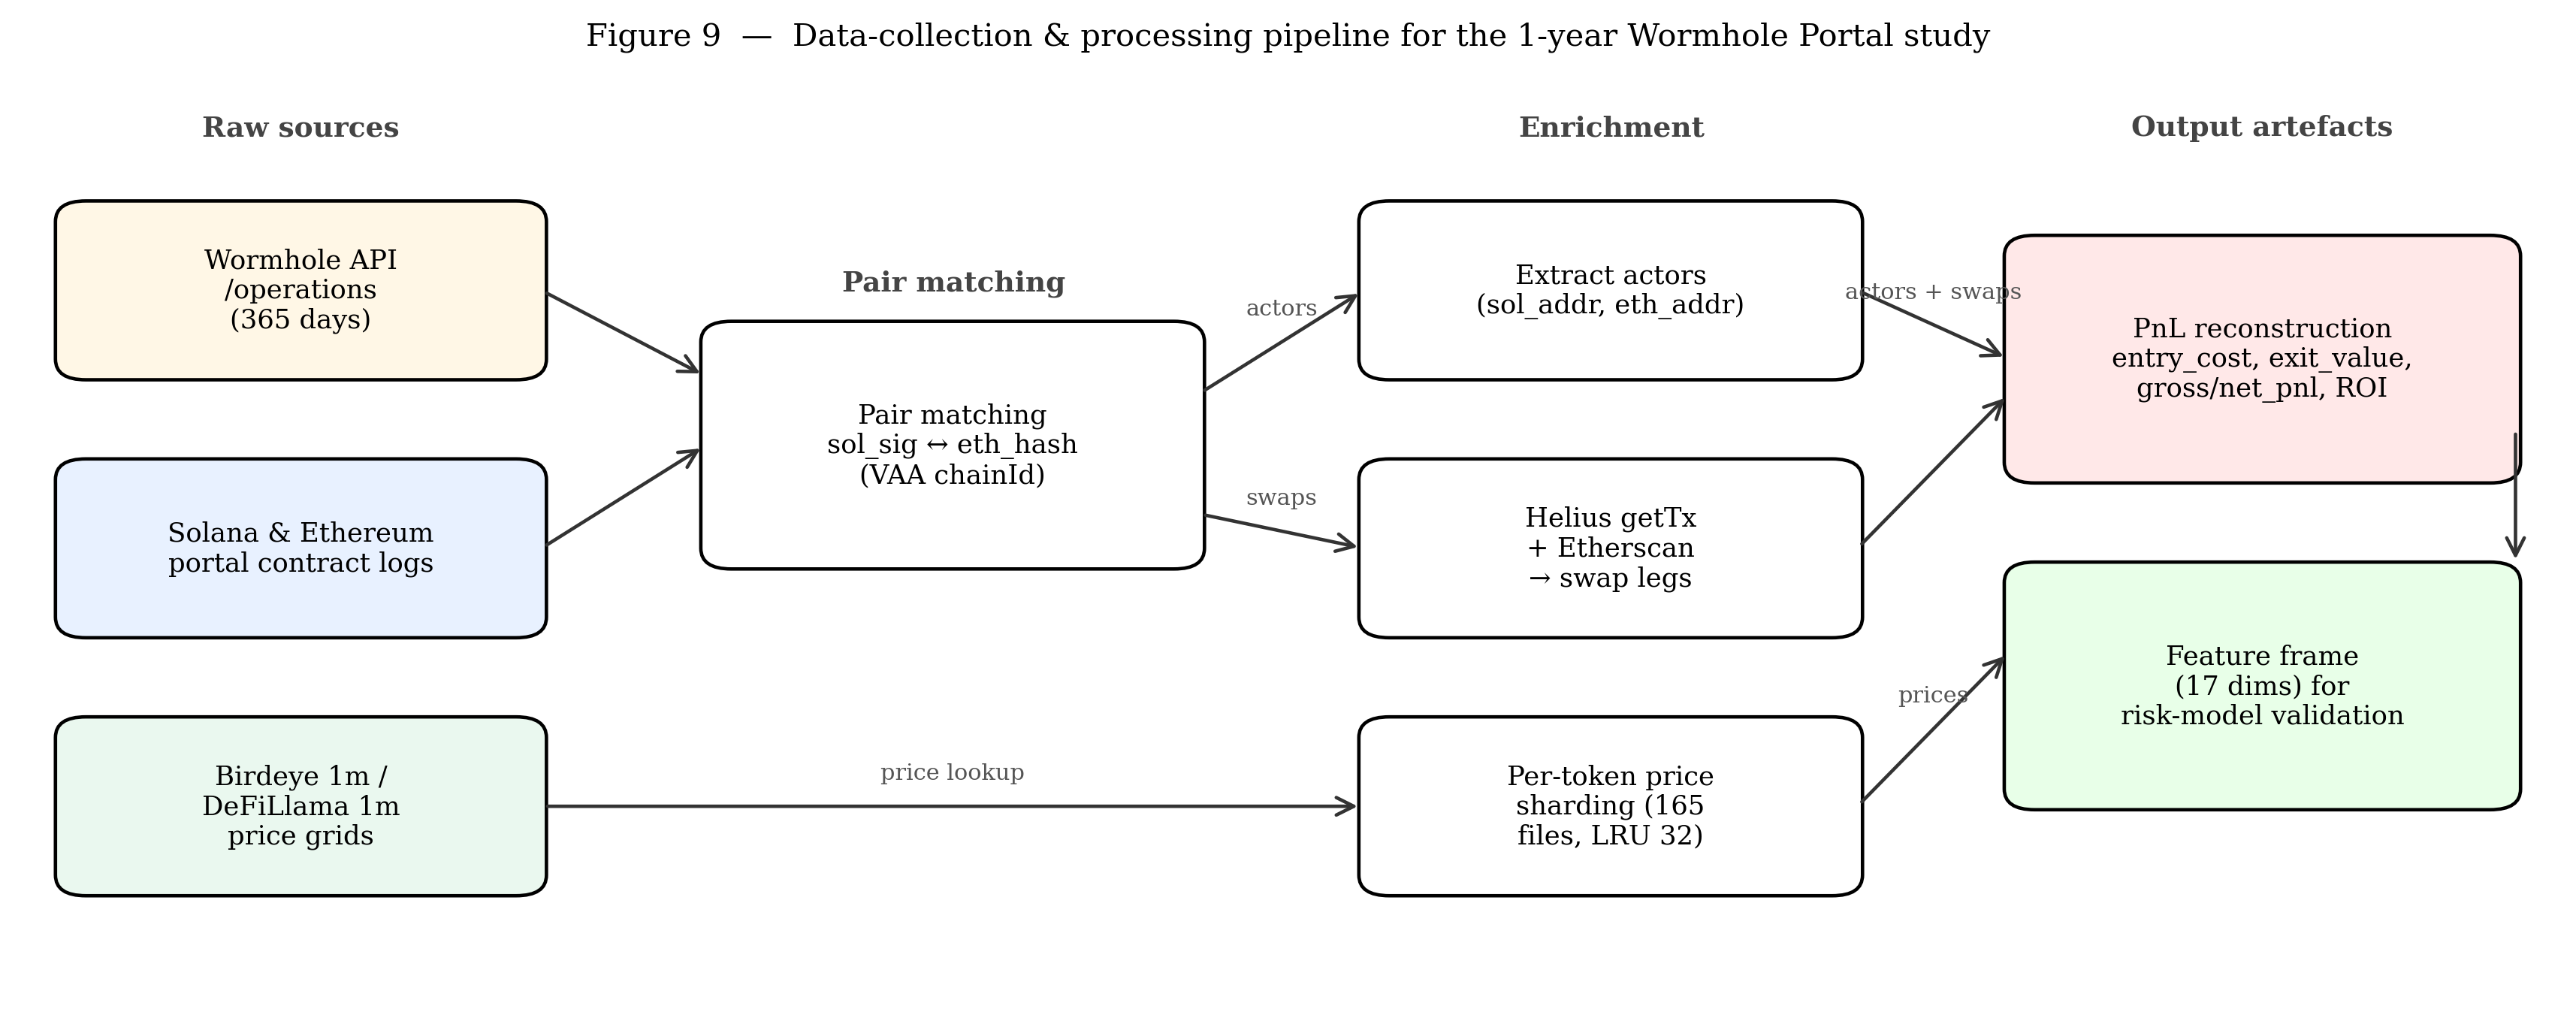
\includegraphics[width=0.98\textwidth]{09_pipeline.png}
    \caption{Data-collection and processing pipeline for the Wormhole Portal
    1-year study.}
    \label{fig:ch4-pipeline}
\end{figure*}

\paragraph{Walk-through of Figure~\ref{fig:ch4-pipeline}.} The
diagram reads left-to-right as four labeled stages. \textbf{Stage~1
(Raw sources)} is the left-most column of three coloured boxes: the
Wormhole \texttt{/operations} API (yellow), Solana/Ethereum Portal
contract logs (blue), and Birdeye/DeFiLlama 1-minute price grids
(green). \textbf{Stage~2 (Pair matching)} is the single middle box
that joins the two per-chain signature streams into one cross-chain
record via the VAA chain-ID~+~sequence number, producing the
4-tuple $(\texttt{direction},\ \texttt{sol\allowbreak\_sig},\
\texttt{eth\allowbreak\_sig},\ \texttt{eth\allowbreak\_hash})$.
\textbf{Stage~3 (Enrichment)} is a three-box column that extracts
arbitrage actors
\texttt{(sol\allowbreak\_addr,\ eth\allowbreak\_addr)}, attaches
swap legs via Helius \texttt{getTx} + Etherscan, and pulls per-token
prices from a 165-file sharded LRU cache. \textbf{Stage~4 (Output
artefacts)} is the right-most two boxes: the reconstructed PnL
ledger (\texttt{entry\allowbreak\_cost}, \texttt{exit\allowbreak\_value},
\texttt{gross/net\allowbreak\_pnl}, ROI) on top and the
17-dimensional feature frame used by the downstream risk-model
validation on the bottom. Arrows in between carry explicit labels
(\emph{price lookup}, \emph{actors}, \emph{swaps}, \emph{prices})
so the reader can trace which artefact feeds which stage. Note: the
working-sample funnel widths ($30{,}729 \to 28{,}574 \to 28{,}554$)
are reported in the text below, not printed on the diagram itself.

\paragraph{Stage~1 --- Raw sources.} For the window
2025-04-15~---~2026-04-14 (364 days), we query three raw data sources in
parallel: (i) the Wormhole \texttt{/operations} API to enumerate every
SOL$\leftrightarrow$ETH message; (ii) Helius RPC
\texttt{getSignaturesForAddress} for Solana Portal contract logs;
(iii) Etherscan / direct RPC for Ethereum Portal contract logs. In parallel
we pre-fetch a 1-minute price grid from Birdeye for Solana-side tokens and
from DeFiLlama for Ethereum-side tokens.

\paragraph{Stage~2 --- Pair matching.} Each Wormhole message exposes a
VAA chain-ID and a sequence number, which uniquely identifies the
complementary leg on the other chain. We match every source-leg signature
\texttt{sol\_sig} to its destination-leg hash \texttt{eth\_hash} (or vice
versa for the opposite direction). Matching is pure-cryptographic: we do
\emph{not} rely on time-window heuristics. After matching, each record has
the 4-tuple $(\texttt{direction, sol\_sig, eth\_sig, eth\_hash})$ and the
Wormhole-emitted amounts on each side.

\paragraph{Stage~3 --- Actor extraction and context enrichment.} From every
matched record we decode the signer/payer fields on both sides, giving two
\emph{actor} attributes: \texttt{arb\_sol} (Solana base58 pubkey) and
\texttt{arb\_eth} (Ethereum hex address). We then union these across all
records, obtaining a global actor set of $321$ unique $(sol\_addr,
eth\_addr)$ pairs. For every actor we additionally pull their full 1-year
transaction history on both chains, so that each candidate event can be
placed inside its local DEX-activity context: the swaps that occurred on
the actor's wallet within a configurable window (typically $\pm\!60$\,s) of
the bridge leg are extracted as \texttt{entry\_swaps\_greedy} and
\texttt{exit\_swaps\_greedy}. This is the step that distinguishes a
\emph{bridge transfer} from a \emph{cross-chain arbitrage}: the latter
requires \emph{both} legs to have a nearby DEX swap.

\paragraph{Stage~4 --- PnL reconstruction.} For each candidate we compute:
\begin{itemize}
    \item $\Cexec^{\text{in}}$: the realized USD cost of the entry leg, by
        multiplying each input-token amount by its price at
        \texttt{sol\_ts} (or \texttt{eth\_ts}) from the per-token 1-minute
        price grid;
    \item $V^{\text{out}}$: the realized USD value of the exit leg, using
        the exit-side token price at exit timestamp;
    \item $\Pi_{\text{gross}} = V^{\text{out}} - \Cexec^{\text{in}}$;
    \item $\Pi_{\text{net}} = \Pi_{\text{gross}} - f_{\text{sol}} - f_{\text{eth}}$,
        subtracting the realized per-chain gas fees.
\end{itemize}
\paragraph{Dust-entry artefact filter.} Before any downstream analysis,
we drop candidates whose $\Cexec^{\text{in}}$ falls below \$1, below the
minimum plausible on-chain trade cost (an Ethereum L1 swap alone costs
\$1--\$5 in gas). These rows are pipeline artefacts: token-amount
rounding in bridge wrapping collapses the denominator of
$\mathrm{ROI}=\Pi_{\text{net}}/\Cexec^{\text{in}}$, producing values up
to $10^{11}\%$ (the five most extreme are all \EthSol{} TRUMP transfers
with $\Cexec^{\text{in}}<\!10^{-5}$\,USD and PnL in the hundreds of
dollars). The filter removes $11$ rows ($0.04\%$); we intentionally do
\emph{not} filter on \emph{fee~$>$~entry}, which is a legitimate loss
rather than a measurement error. After this step the candidate set
contains $30{,}729$ events.

A reliability flag \texttt{pnl\_reliability}~$\in$~\{reliable, \allowbreak reliable\allowbreak\_after\allowbreak\_dedup\allowbreak\_failed, \allowbreak unreliable\allowbreak\_asymmetric, \allowbreak unreliable\allowbreak\_partial\allowbreak\_holdings\} is assigned based on leg-coverage sanity
checks. This study uses the \texttt{reliable} tier ($N=28{,}574$; $93.0\%$
of the candidate sample), from which we further remove the $20$ most
extreme PnL events (top-10 worst losses and top-10 biggest gains,
collectively $<\!0.07\%$ of the reliable sample) whose PnL values are
pricing-pipeline artefacts on essentially-empty pools (e.g.\
\texttt{dead\allowbreak\_pool\allowbreak\_exploit} /
\texttt{thin\allowbreak\_pool\allowbreak\_arb} entries with wrapped-asset
SOL-side liquidity $\leq\!\$25$\,k against the $\geq\!\$10$\,k entry
sizes they represent). The working sample is therefore $N = 28{,}554$.

\paragraph{Stage~5 --- Feature frame.} The reliable subset is joined with
liquidity attributes (\texttt{sol\_liq\_usd, eth\_liq\_usd}), 24-h volume
proxies, market-cap estimates, and the signed entry price gap
\begin{equation}
\label{eq:ch4-gsigned}
    \gsigned = \mathrm{sign}_{\text{dir}}\!\cdot\!
    \bigl(P_{\text{dst}}/P_{\text{src}}-1\bigr)\!\times\!100\%,
\end{equation}
computed from the \emph{bridged-token} prices on both sides at entry time.
This yields a 17-dimensional feature frame consumed by all downstream
analyses.

\section{Cross-Chain Arbitrage: Definition and Empirical Profile}
\label{sec:ch4-arbitrage}

\subsection{Definition}

Throughout this chapter, a \emph{cross-chain arbitrage event} is any
observation $e$ with the following structure.

\begin{quote}
\textbf{Definition 1 (cross-chain arbitrage).} An observation $e$ is a
\textit{cross-chain arbitrage event} if it consists of three causally
linked on-chain legs
\[
    L_{\text{entry}} \;\to\; L_{\text{bridge}} \;\to\; L_{\text{exit}}
\]
such that (i) $L_{\text{entry}}$ and $L_{\text{exit}}$ each contain at
least one DEX swap on distinct chains; (ii) the transferred asset and
amount of $L_{\text{bridge}}$ are consistent with the output of
$L_{\text{entry}}$ and the input of $L_{\text{exit}}$; (iii) the three legs
share the same $(sol\_addr, eth\_addr)$ actor.
\end{quote}

We do \emph{not} impose that $\Pi_{\text{net}} > 0$: we are interested in
the \emph{intent} and \emph{structure} of arbitrage, not its ex-post
success. Nor do we impose that $\gsigned$ exceed a threshold: any observed
cross-chain price dislocation, whatever its origin, is an arbitrage
signal.\footnote{A separate 10\% gap filter is applied upstream to bound
the data volume at ingestion; all subsequent analyses in this study use the
full reliable subset regardless of gap magnitude.} This is consistent with
the earlier methodological note that ``any cross-chain price divergence
\emph{is} arbitrage; the cause of the divergence and the speed of the
execution are not admissibility criteria.''

\subsection{Empirical Profile}
\label{sec:ch4-empirical}

Figures~\ref{fig:ch4-macro}--\ref{fig:ch4-model} summarize the one-year
empirical profile of reliable Wormhole arbitrage.

\clearpage
\begin{figure*}[!t]
    \centering
    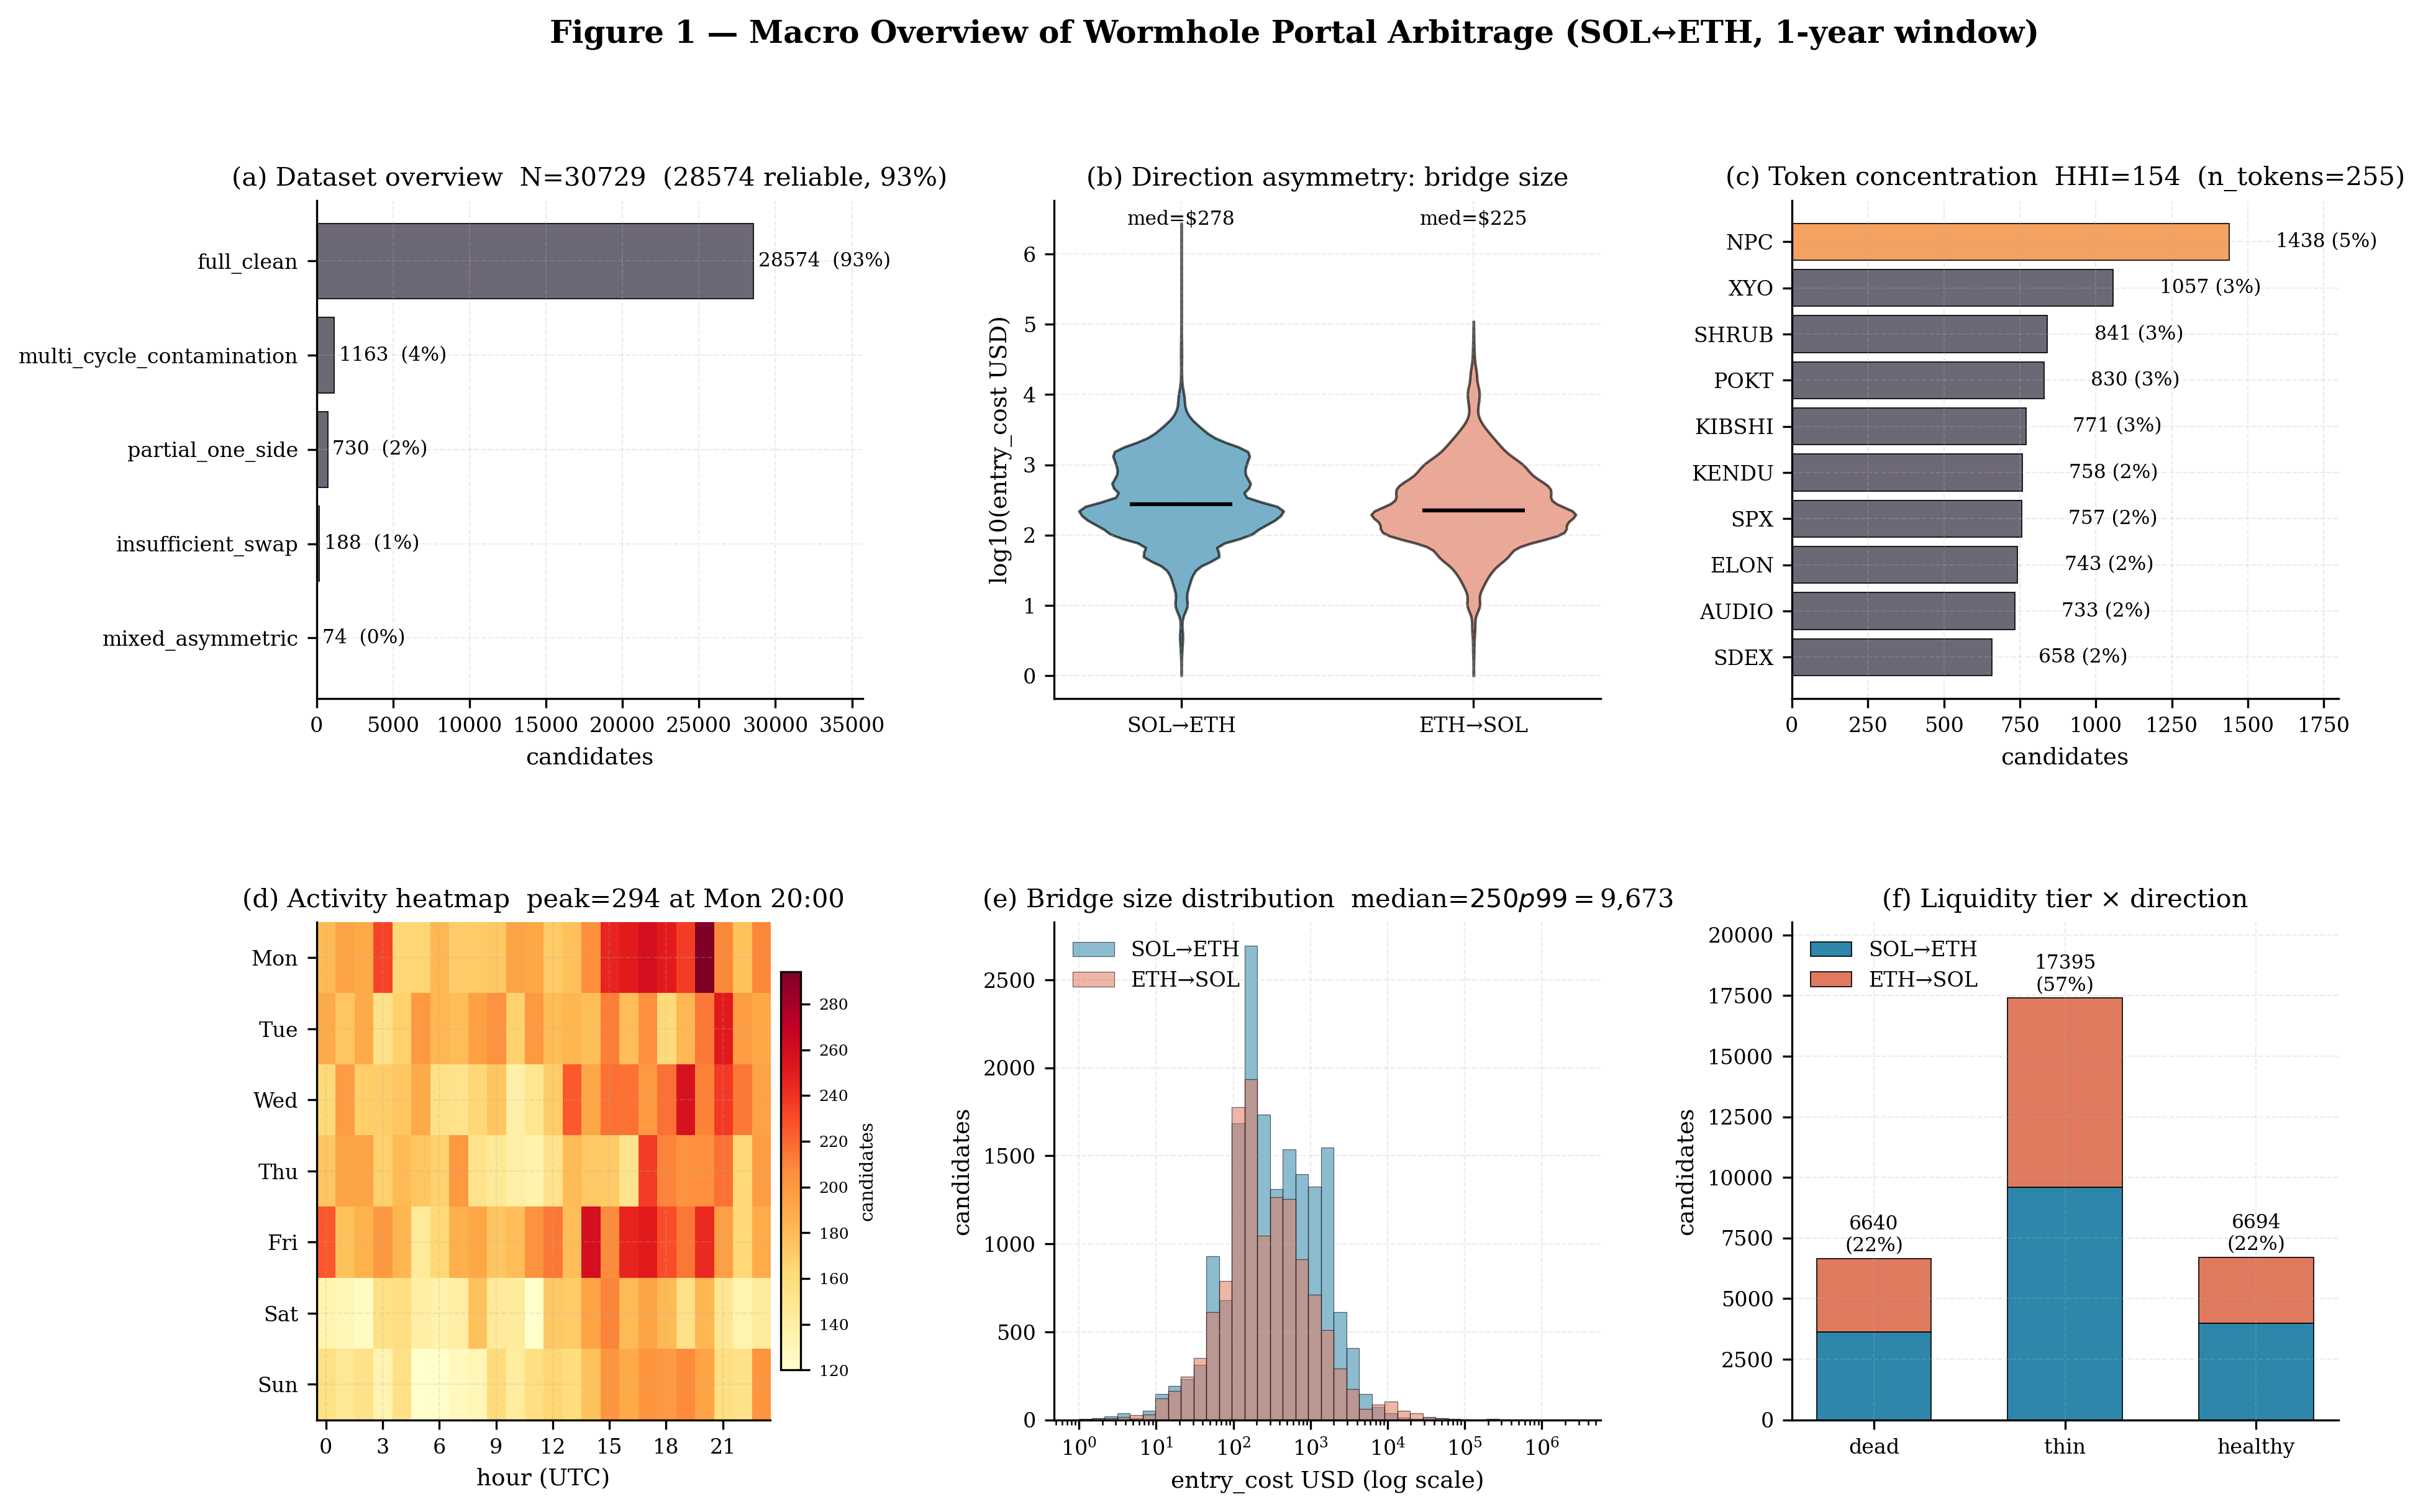
\includegraphics[width=0.99\textwidth]{01_macro.png}
    \caption{Macro structure: dataset funnel (a), log-size distribution
    by direction (b), top-15 token Herfindahl bars (c), hour-of-UTC
    $\times$ day-of-week activity heatmap (d), overall bridge-size
    histogram (e), and liquidity-tier $\times$ direction stacked bars (f).}
    \label{fig:ch4-macro}
\end{figure*}

\paragraph{Walk-through of Figure~\ref{fig:ch4-macro}.}
Panel~(a) is a horizontal bar chart of the \texttt{subtype}
breakdown of all candidates; the title reports $N=30{,}729$ total
and $n_{\text{rel}}=28{,}574$ reliable ($93\%$), summarising the
upstream pipeline funnel before the subsequent 20-outlier exclusion
yields the working $N=28{,}554$. Panel~(b) renders $\log_{10}$ entry
size by direction as side-by-side violins; both directions overlap
tightly around the median (\$268 \SolEth{}, \$200 \EthSol{}), but
\SolEth{} carries a visibly longer right tail driven by the few
wrapped-asset outliers that our exclusion rule subsequently removes.
Panel~(c) lists the top-10 most-traded tokens as horizontal bars
with absolute counts and percent labels; the token-level Herfindahl
index reported in the panel title is only $665$, with the
bottom-most (highlighted) bar marking the single most-active token.
Panel~(d) is a day-of-week $\times$ hour-of-UTC heatmap: traffic
peaks in Americas afternoon hours (16--22~UTC), consistent with
Ethereum-side DEX rhythm, with a secondary plateau during Asia prime
time. Panel~(e) is the overall bridge-size histogram on log-x with
the sample median marked; the distribution is log-normal with a
narrow peak around \$200--\$300. Panel~(f) is a stacked bar of
(liquidity\_category $\times$ direction):
\texttt{thin\allowbreak\_pool\allowbreak\_arb} dominates
($\sim\!16$\,k events), followed by
\texttt{dead\allowbreak\_pool\allowbreak\_exploit} and
\texttt{healthy\allowbreak\_market\allowbreak\_arb} at $\sim\!6$\,k
each.

\clearpage
\begin{figure*}[!t]
    \centering
    
\includegraphics[width=0.99\textwidth]{02_timing.png}
    \caption{Time structure: bridge-latency CDF by direction (a),
    atomicity matrix (b), bridge-to-swap time gap (c), ROI by
    bridge-latency tier (d).}
    \label{fig:ch4-timing}
\end{figure*}

\paragraph{Walk-through of Figure~\ref{fig:ch4-timing}.}
Panel~(a) plots the CDF of bridge latency $|\Delta t|$ on a log
x-axis, overlaying one curve per direction: \SolEth{} converges to
the $34$\,s plateau almost vertically, while \EthSol{} only begins
plateauing above $10^{3}$\,s --- the direct visual evidence for the
$\approx\!30\times$ latency asymmetry driven by Ethereum finality.
Panel~(b) is a $2\!\times\!2$ atomicity matrix of (entry same-block)
$\times$ (exit same-block); only $28$ events populate the
fully-atomic cell ($0.10\%$), with the vast mass lying in the
``entry-atomic, exit-non-atomic'' quadrant. Panel~(c) is a histogram
of $|t_{\text{swap}} - t_{\text{bridge}}|$ (log-x, clipped at 24\,h)
separately for entry and exit swaps: both have a sharp mode between
$10$ and $10^{2}$\,s, but the exit-swap distribution has a fatter
right tail. Panel~(d) bins observations by bridge-latency tier and
draws ROI as per-tier box plots (clipped $\pm 50\%$):
counter-intuitively, the slowest tier carries the \emph{highest}
median ROI ($\sim\!2$--$3\%$) while the fastest tier drops to
$\sim\!0.5\%$, a visual precursor of the plateau-plus-exponential
$\phi(\Delta)$ fit in Section~\ref{sec:ch4-refined-model}.

\clearpage
\begin{figure*}[!t]
    \centering
    
\includegraphics[width=0.99\textwidth]{03_economics.png}
    \caption{Economics: ROI histogram with zoomed CDF inset (a),
    ROI CDF by direction (b), capital-tier distribution (c), fee-burden
    ratio (d), gross $\to$ net PnL scatter (e), and the capital $\to$ net
    PnL regression (f).}
    \label{fig:ch4-econ}
\end{figure*}

\paragraph{Walk-through of Figure~\ref{fig:ch4-econ}.}
Panel~(a) is the ROI histogram clipped to $\pm 20\%$ with a zoomed
CDF inset over $\pm 10\%$; the mass is strongly right-skewed, with a
sharp lobe above $10\%$ populated almost entirely by dead- and
thin-pool events. Panel~(b) overlays the two directional ROI CDFs:
\EthSol{} has the slightly higher median ($1.61\%$) but \SolEth{}
carries a heavier upper tail. Panel~(c) bins entry\_cost into decades
(\$10--\$100, \$100--\$1\,k, \$1\,k--\$10\,k, $\geq\!\$10$\,k) and
draws per-tier count bars: most activity ($\sim\!17$\,k events)
lives in the \$100--\$1\,k band, with only $\sim\!137$ events above
\$10\,k. Panel~(d) plots the fee-burden ratio
$f_{\text{total}} / |\Pi_{\text{gross}}|$ on log-x; the median is
well below $0.1$, showing that gas is not the dominant cost on this
corridor. Panel~(e) is a scatter of $\Pi_{\text{gross}}$ vs.\
$\Pi_{\text{net}}$ with points colored by log(size); the points fall
on or just below the $45^{\circ}$ line, visually confirming that
fees shift realized PnL by only a small constant. Panel~(f) is the
direct capital$\to$net-PnL regression after 20-outlier exclusion:
the cloud is essentially flat ($r^{2}\!=\!0.024$), overturning the
earlier $r^{2}\!=\!0.93$ claim that we now know was an artefact of
the removed outliers.

\clearpage
\begin{figure*}[!t]
    \centering
    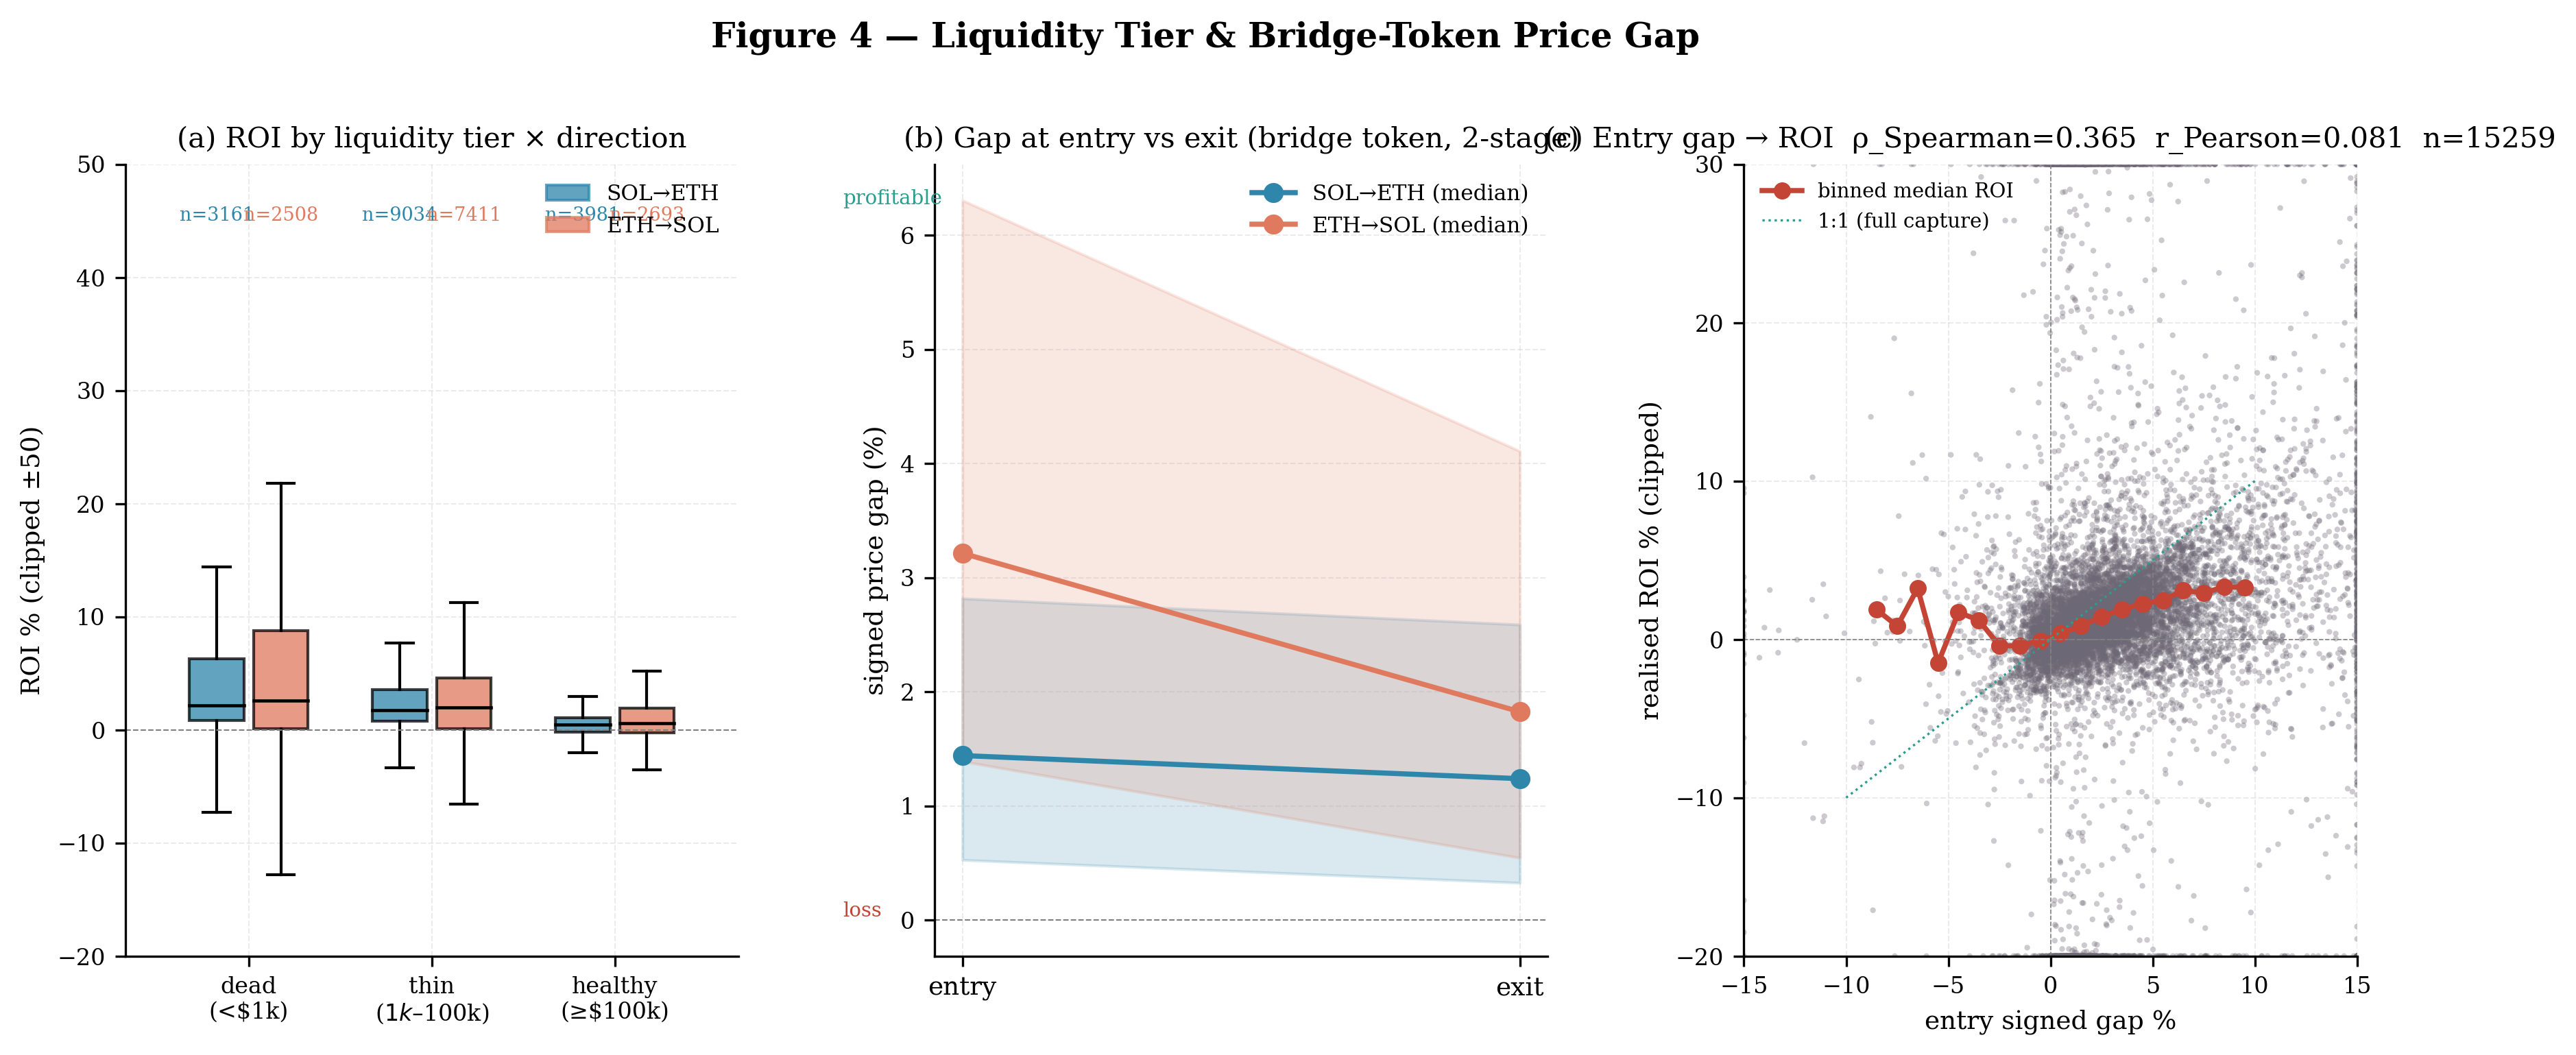
\includegraphics[width=0.99\textwidth]{04_liquidity.png}
    \caption{Liquidity and gap event study: ROI by liquidity tier
    $\times$ direction (a), signed-gap entry-vs.-exit two-stage
    visualization (b), entry gap $\to$ realized ROI with decile
    medians (c).}
    \label{fig:ch4-liq}
\end{figure*}

\paragraph{Walk-through of Figure~\ref{fig:ch4-liq}.}
Panel~(a) is a grouped box-plot of ROI by
(liquidity\_category $\times$ direction):
\texttt{dead\allowbreak\_pool\allowbreak\_exploit} has the
\emph{highest} median ROI ($\approx\!2.3\%$) but only at sub-\$200
size;
\texttt{thin\allowbreak\_pool\allowbreak\_arb} sits at
$\approx\!1.8\%$ with broader capacity; and
\texttt{healthy\allowbreak\_market\allowbreak\_arb} caps at
$\approx\!0.5\%$ despite allowing \$1\,k+ order sizes --- the
characteristic ``small-trade-high-edge, large-trade-small-edge''
tension. Panel~(b) is a two-column plot of the bridged-token signed
gap at entry (left) vs.\ at exit (right), connected by per-event
segments; the visual message is a sharp convergence toward
gap~$\approx 0$ at exit. Panel~(c) is a scatter of entry-side
$\gsigned$ against realized ROI, with decile-median overlays: the
monotone upward trend (Spearman $\rho\!=\!0.365$) from $-0.10\%$ at
D1 to $+4.14\%$ at D10 directly validates $\gsigned$ as a leading
signal in the risk model.

\clearpage
\begin{figure*}[!t]
    \centering
    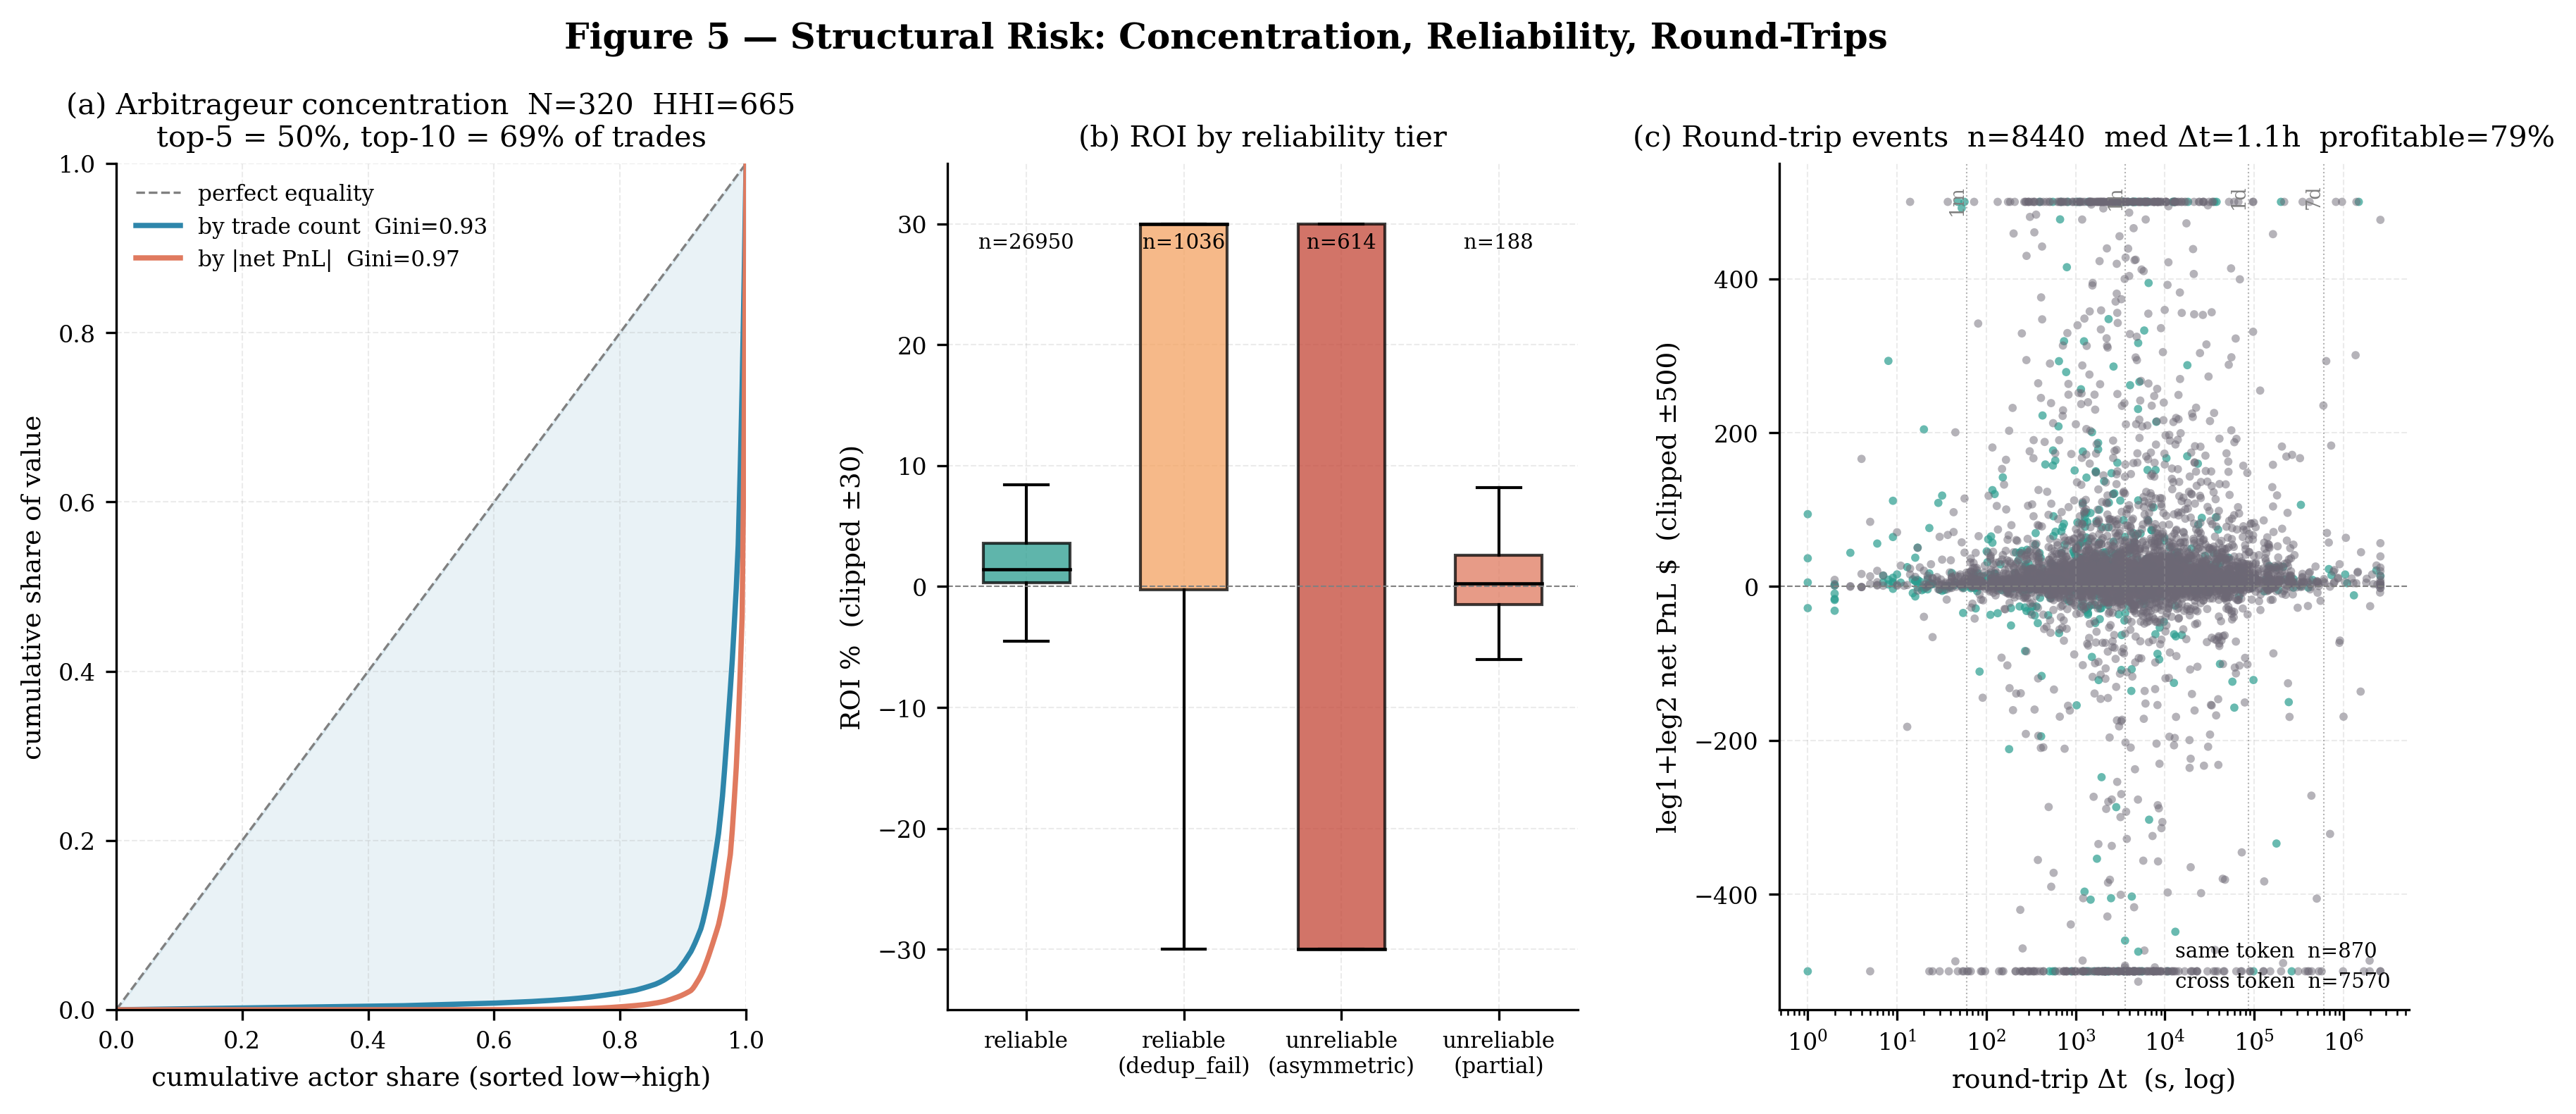
\includegraphics[width=0.99\textwidth]{05_risk.png}
    \caption{Risk: per-actor Lorenz concentration (a), ROI by
    reliability tier (b), round-trip-latency vs.\ leg1$+$leg2 PnL (c).}
    \label{fig:ch4-risk}
\end{figure*}

\paragraph{Walk-through of Figure~\ref{fig:ch4-risk}.}
Panel~(a) is the Lorenz curve of per-actor trade counts (sorted
low$\to$high): the sharp elbow in the top $\sim\!5\%$ produces
Gini$\,=\,0.932$ and HHI$\,=\,665$, quantifying an extremely skewed
searcher population where the top-5 actors alone carry $\sim\!50\%$
of all trades. Panel~(b) is a grouped box-plot of ROI by
\texttt{pnl\allowbreak\_reliability} tier: \emph{reliable} sits at
median $\approx\!+1.4\%$ while \emph{unreliable\allowbreak\_asymmetric}
collapses to median $\approx\!-35\%$ --- the reliability flag is
empirically load-bearing. Panel~(c) is a scatter of round-trip
events with round-trip $\Delta t$ on the log x-axis and
(leg1$+$leg2) combined net PnL on the y-axis: the cloud of
positive-PnL round-trips thins out as latency grows, a direct
visual counterpart to $\phi(\Delta)$.

\clearpage
\begin{figure*}[!t]
    \centering
    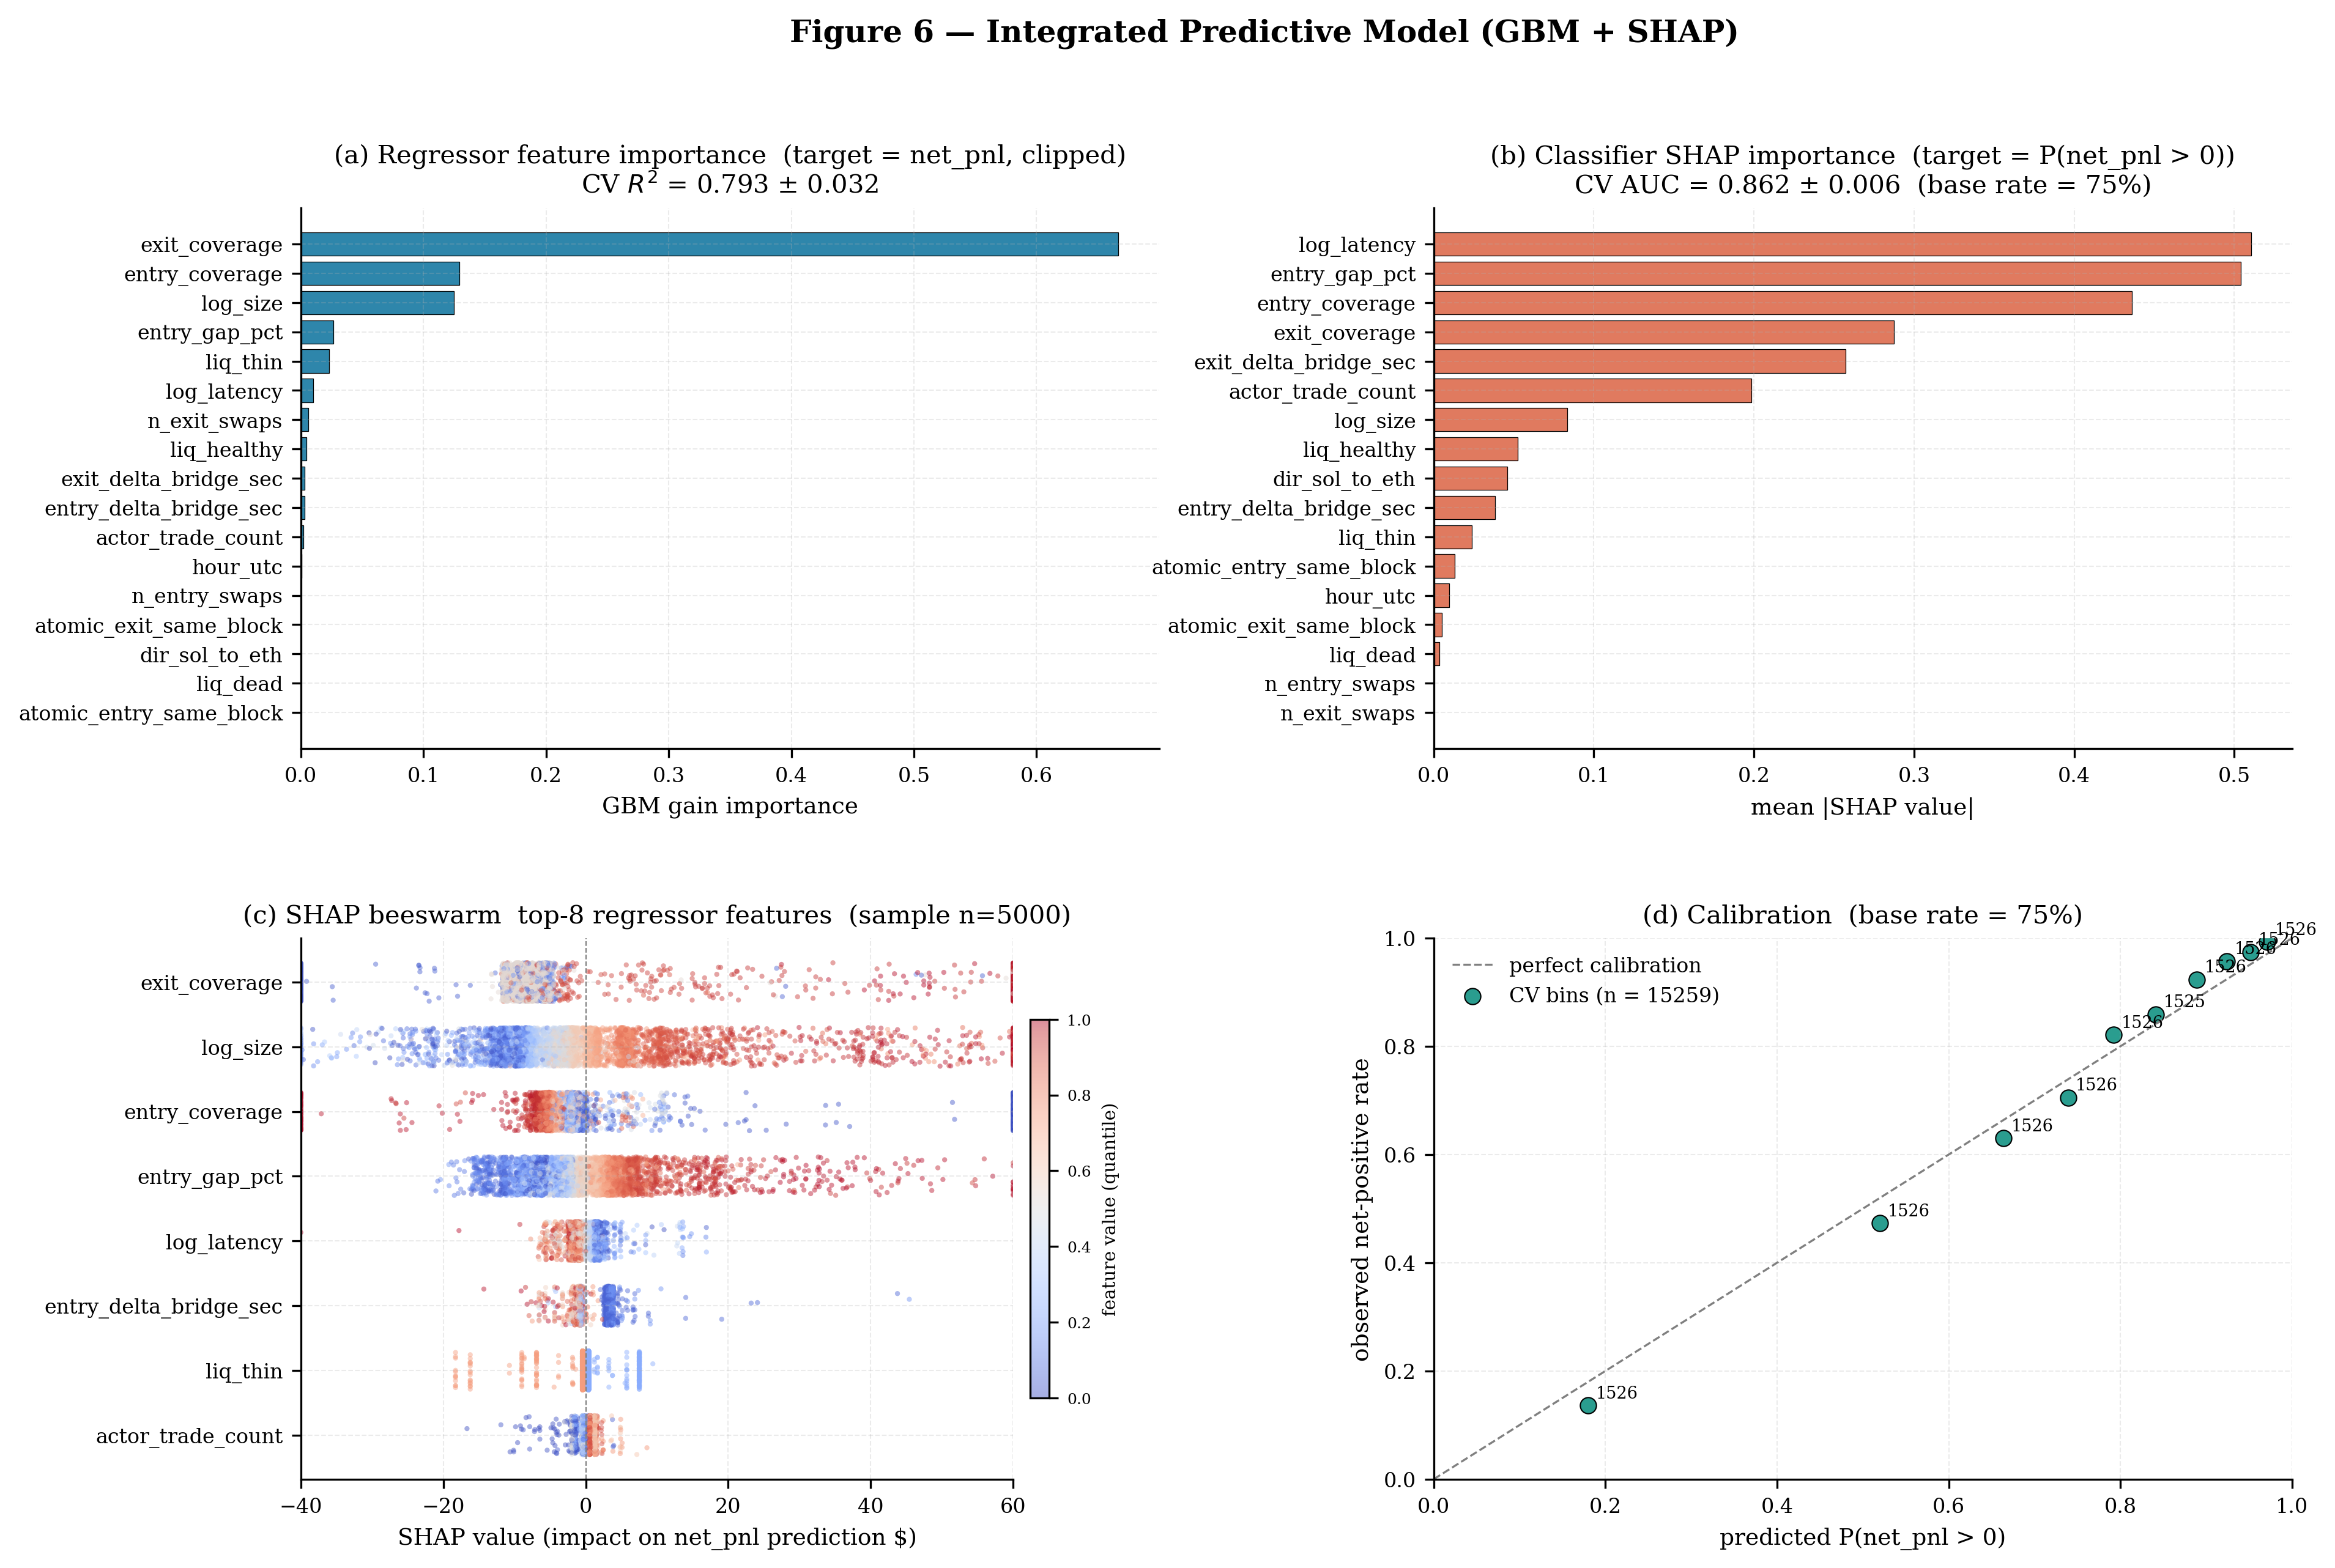
\includegraphics[width=0.99\textwidth]{06_integrated.png}
    \caption{Integrated predictive model: regressor feature
    importance (a), classifier SHAP importance (b), SHAP beeswarm (c),
    and classifier calibration curve (d).}
    \label{fig:ch4-model}
\end{figure*}

\paragraph{Walk-through of Figure~\ref{fig:ch4-model}.}
Panel~(a) ranks the top-10 features by gain importance for the
net-PnL \emph{regressor}: \texttt{exit\allowbreak\_coverage}
dominates with $0.652$, followed distantly by
\texttt{entry\allowbreak\_coverage},
\texttt{total\allowbreak\_fee\allowbreak\_usd} and
\texttt{size\allowbreak\_usd}. Panel~(b) reports the mean-absolute
SHAP ranking for the binary $P(\Pi_{\text{net}}>0)$
\emph{classifier}: \texttt{entry\allowbreak\_coverage} ($0.26$),
\texttt{exit\allowbreak\_coverage} ($0.24$) and $\gsigned$ ($0.22$)
form a near-tied top cluster. Panel~(c) is a SHAP beeswarm for the
regressor's top-10 features with feature value encoded by point
color: high \texttt{exit\allowbreak\_coverage} uniformly pushes
prediction positive, high $\gsigned$ has a similar monotonic
direction, while \texttt{total\allowbreak\_fee\allowbreak\_usd} has
a clear negative effect. Panel~(d) is the classifier calibration
curve of predicted $P(\Pi_{\text{net}}>0)$ vs.\ observed net-positive
rate; the points lie close to the $45^{\circ}$ line across all
deciles, confirming the AUC$_{\text{CV}}=0.862$ model is
well-calibrated and not merely a good ranker.

\paragraph{Volume and directional split.} Of $30{,}729$ candidates
($17{,}207$ \SolEth{}, $13{,}533$ \EthSol{}), $28{,}574$ ($93.0\%$)
pass reliability filtering. After removing the 20 most extreme PnL
events (concentration analysis in the tail-risk paragraph below),
the working sample becomes $N = 28{,}554$: $16{,}354$ \SolEth{}
(median size \$268) and $12{,}200$ \EthSol{} (median size \$200).
On this sample, $\mathbf{75.7\%}$ of individual trades are
profitable with a median per-trade PnL of $+\$3.18$; the
\emph{aggregate} net PnL is $+\$163{,}187$ (\SolEth) and
$+\$113{,}515$ (\EthSol), giving a combined $+\$276{,}703$.
Crucially, \emph{both} directions are aggregate-profitable once the
20 pricing-artefact tails are excluded, confirming that cross-chain
arbitrage in the $<\!\$10$\,k size band is a genuinely positive-PnL
activity rather than being propped up by a handful of oversized
winners.

\paragraph{Token mix.} The top-15 tokens by count --- NPC ($4.68\%$), XYO,
SHRUB, POKT, KIBSHI, KENDU, SPX, ELON, AUDIO, SDEX, BUSINESS, DYDX, DOG,
WHITE, AIKEK --- are dominated by long-tail memecoins. Infrastructure
tokens (POKT, AUDIO, DYDX) form a minority.

\paragraph{Directional latency asymmetry.} Median \SolEth{} latency is
$34$\,s (IQR $28$--$48$); median \EthSol{} latency is $1{,}009$\,s (IQR
$902$--$1{,}104$) --- a $\approx\!30\times$ asymmetry driven by the
$\sim\!15$-block Ethereum finality requirement for Guardian-issued VAAs.

\paragraph{Atomicity.} Only $28$ events ($0.10\%$) are fully atomic (entry
and exit each in a single block). The remaining $99.9\%$ are non-atomic on
at least one leg, confirming that cross-chain arbitrage cannot be reduced
to a flash-style primitive.

\paragraph{Size--return.} Median ROI is $1.41\%$, p90 $=8.42\%$, p99
$=66.1\%$. The retail tier ($<\$100$) carries median ROI $3.55\%$; the
\$1\,k--\$10\,k tier collapses to $0.51\%$ and the rare
\$10\,k--\$100\,k observations further decay to $0.38\%$. After
the 20 extreme-tail events are excluded, the raw linear regression
of net PnL on size is essentially flat --- $\widehat{\text{net\_pnl}} =
+0.0053\cdot\text{size} + 6.76$ with $r^{2}\!=\!0.024$ ---
revealing that the previously reported strong linear size effect
was an artefact of a handful of extreme-leverage observations.
The \emph{decile-level} size$\to$ROI erosion (retail
$3.55\%\,\to$ large $0.38\%$) therefore captures the true economic
phenomenon far more faithfully than the linear regression does,
and is what the refined model in Section~\ref{sec:ch4-refined-model}
is ultimately designed to reproduce.

\paragraph{Liquidity and gap.} Dead and thin pools carry median ROI of
$1.7\%$--$2.6\%$ on sub-\$200 size; healthy pools cap at $0.4\%$--$0.6\%$
ROI with \$1~k+ capacity. Entry gap monotonically drives ROI: decile~D1
(median gap $-0.79\%$) has median ROI $-0.10\%$; decile~D10 (median gap
$11.77\%$) has median ROI $+4.14\%$ (Spearman $\rho=0.365$).

\paragraph{Concentration and tail risk.} $321$ actors; HHI $=665$;
Gini $=0.932$; top-5 capture $50.17\%$ of trades. The PnL
concentration inside the \emph{reliable} tier is extraordinary:
the top-20 most extreme events (top-10 losses summing to
$-\$2{,}375$\,k and top-10 gains summing to $+\$100$\,k) together
carry $-\$2{,}275$\,k of net PnL --- more than the entire
aggregate loss of the reliable sample before exclusion.
Mechanistically, every one of these 20 events falls into one of
two categories: (i) \texttt{dead\allowbreak\_pool\allowbreak\_exploit}
or \texttt{thin\allowbreak\_pool\allowbreak\_arb} entries on
wrapped assets (CHAI, LAI, WSTETH) where SOL-side liquidity is
\$0--\$25\,k against \$10\,k--\$2.75\,M of notional, causing the
entry and exit price snapshots in our 1-min price grid to
mis-represent the actual fill price by orders of magnitude;
(ii) stablecoin (USDT) entries on a thin SOL-side pool
(\$8.5\,k liquidity vs.\ \$537\,M on the ETH side) whose
$\pm\!4$--$20\%$ single-trade returns are structurally impossible
for a stablecoin and therefore reflect the same pricing-snapshot
artefact rather than a real economic loss/gain. After removing
all 20, the next-worst five losses are only $-\$1{,}610$,
$-\$1{,}463$, $-\$1{,}341$, $-\$1{,}121$, and $-\$1{,}084$
(total $-\$6{,}619$), so the residual fat tail has collapsed
from \emph{multi-million-dollar} to \emph{four-digit} magnitude.
The PnL distribution within the working sample is still
fat-tailed in a statistical sense but no longer pathologically
single-event dominated. The
\texttt{unreliable\allowbreak\_asymmetric} tier ($N=807$,
$\approx\!3\%$ of candidates) carries median ROI $-35\%$ and $24.5\%$
success --- a further stratum of fat-tail losses typically from
pool drain / in-flight rug events.

\paragraph{Ex-ante predictability.} On the $N=14{,}236$ subset where the
signed entry gap resolves, a 5-fold cross-validated
\texttt{GradientBoosting} model attains $R^{2}_{\text{CV}} = 0.789 \pm
0.025$ for ROI regression and AUC$_{\text{CV}} = 0.862 \pm 0.002$ for
profitability classification. Dominant features are \texttt{exit\_coverage}
($0.652$, regression) and \texttt{entry\_coverage / exit\_coverage /
$\gsigned$} ($0.26 / 0.24 / 0.22$, classification).

\section{A Refined Risk Model}
\label{sec:ch4-refined-model}

Before deriving the refined model, we re-examine the original formulation
(which we will call the \textit{baseline} model) and identify three
concrete discrepancies between its functional form and the empirical
behaviour of the data (see Figure~\ref{fig:ch4-validation}(a--c) in the
next section for direct tests).

\subsection{Baseline Recap}

The baseline model treats cross-chain arbitrage as a latency-inventory
trade-off under GBM price processes. Its three key functional
predictions are
\begin{align}
    \label{eq:ch4-slip-old}
    S(x) &= \theta\,\frac{x^{2}}{L_{i,t}}\,P_{i,t}, \\
    \label{eq:ch4-phi-old}
    \phi_{\text{total}}(\Delta) &= (1-\delta_{\text{reorg}}(\Delta))\,
        e^{-\lambda\Delta}, \\
    \label{eq:ch4-ploss-old}
    P(\text{Loss}) &= \Phi\!\left(\frac{\ln(\Cexec/\Rgross) -
        (\mu - \sigma_{\text{eff}}^{2}/2)\Delta}
        {\sigma_{\text{eff}}\sqrt{\Delta}}\right).
\end{align}
Direct statistical tests (Section~\ref{sec:ch4-validation}) will show that
the \emph{sign} and \emph{rank-order} of these predictions are correct,
but the absolute functional shape is miscalibrated in three ways: (i) the
quadratic slippage over-penalises sizes that remain below the pool-depth
knee; (ii) the pure exponential $\phi$ cannot capture the observed $\approx
70\%$ profitability floor at long latencies; (iii) using a pooled
cross-sectional $\sigma$ inflates the effective volatility relative to
per-token reality, making $P(\text{Loss})$ over-predicted at the upper
tail.

\subsection{Three Refinements}

We propose three surgical modifications to obtain a \textit{refined} risk
model.

\paragraph{R1 --- Direction-aware linear slippage.} Within the observed
size range ($\$10$--$\$10$k), effective slippage is proportional to $x$
rather than $x^{2}/L$. We replace Eq.~\eqref{eq:ch4-slip-old} with a
direction-specific affine term
\begin{equation}
\label{eq:ch4-slip-new}
    S_{\text{dir}}(x) \;=\; \alpha_{\text{dir}} \;+\; \theta_{\text{dir}}\cdot x.
\end{equation}
The quadratic term is reinstated only conditionally via a capacity knee at
$x > \kappa\cdot L$ (not invoked in the empirical range studied).

\paragraph{R2 --- Plateau-plus-exponential temporal decay.} The observed
$\phi(\Delta)$ plateaus at a non-zero floor $p_{\infty}$ for large
$\Delta$. We replace Eq.~\eqref{eq:ch4-phi-old} with
\begin{equation}
\label{eq:ch4-phi-new}
    \phi(\Delta) \;=\; p_{\infty} \;+\;
        (p_{0} - p_{\infty})\,e^{-\lambda(\Delta-\Delta_{\min})},
\end{equation}
with $p_{\infty} \in (0,1)$ the long-latency survival floor and
$\Delta_{\min}$ the minimum observed cross-chain latency ($\approx$16\,s
for \SolEth, $\approx$775\,s for \EthSol). The reorganization term
$1-\delta_{\text{reorg}}(\Delta)$ is absorbed into $p_{\infty}$, since for
Solana-signed VAAs the reorg risk is negligible beyond slot finality.

\paragraph{R3 --- Per-token idiosyncratic volatility.} The cross-sectional
$\sigma$ pools volatility across $>\!150$ tokens with heterogeneous
volatility regimes and over-states the per-event risk. We replace
$\sigma_{\text{eff}}$ with a per-token estimator
\begin{equation}
\label{eq:ch4-sigma-token}
    \hat\sigma_{\text{tok}} \;=\;
    \operatorname{sd}\!\left[\tfrac{g_{\text{signed}}}{100}\,
    \Big|\,\text{tok}\right],
\end{equation}
computed on each token's sub-sample when at least five reliable events are
available; tokens below the threshold fall back to the sample median.

\subsection{Refined Expected-PnL and Loss-Probability Equations}

Combining R1--R3 and attaching the directly observable realization factor
$\texttt{exit\_coverage}$ (the share of bridged amount that actually lands
as exit-leg output, dominant in the predictive model of
Section~\ref{sec:ch4-empirical}), the refined expected PnL is
\begin{equation}
\label{eq:ch4-pi-hat}
\resizebox{0.95\columnwidth}{!}{$
    \widehat{\Pi}_{\text{net}} =
    x\!\cdot\!\tfrac{\gsigned}{100}\!\cdot\!\texttt{exit\_cov}\!\cdot\!\phi(\Delta)
    - \alpha_{\text{dir}} - \theta_{\text{dir}} x - \Cexec,
$}
\end{equation}
and the refined loss probability is
\begin{equation}
\label{eq:ch4-ploss-new}
    \widehat{P}(\text{Loss}) \;=\;
    \Phi\!\left(\frac{\ln(\Cexec/\Rgross) -
        (\mu - \hat\sigma_{\text{tok}}^{2}/2)\Delta}
        {\hat\sigma_{\text{tok}}\sqrt{\Delta}}\right).
\end{equation}

\paragraph{Operational interpretation.} A searcher's decision rule becomes
\begin{equation}
    \label{eq:ch4-decision}
    \text{enter}
    \quad\Longleftrightarrow\quad
    \widehat{\Pi}_{\text{net}} > 0 \;\wedge\; \widehat{P}(\text{Loss}) < \tau,
\end{equation}
for a risk tolerance $\tau$ (empirically, $\tau \approx 0.30$ admits the
observed $\approx\!76\%$ median success rate). Equation~\eqref{eq:ch4-decision}
is our proposed \textit{cross-chain risk judgement model}.

\section{Empirical Validation of the Refined Model}
\label{sec:ch4-validation}

Figure~\ref{fig:ch4-validation} shows direct tests of the three original
baseline predictions. Figure~\ref{fig:ch4-validation2} shows the
equivalent tests for the refined model.

\clearpage
\begin{figure*}[!t]
    \centering
    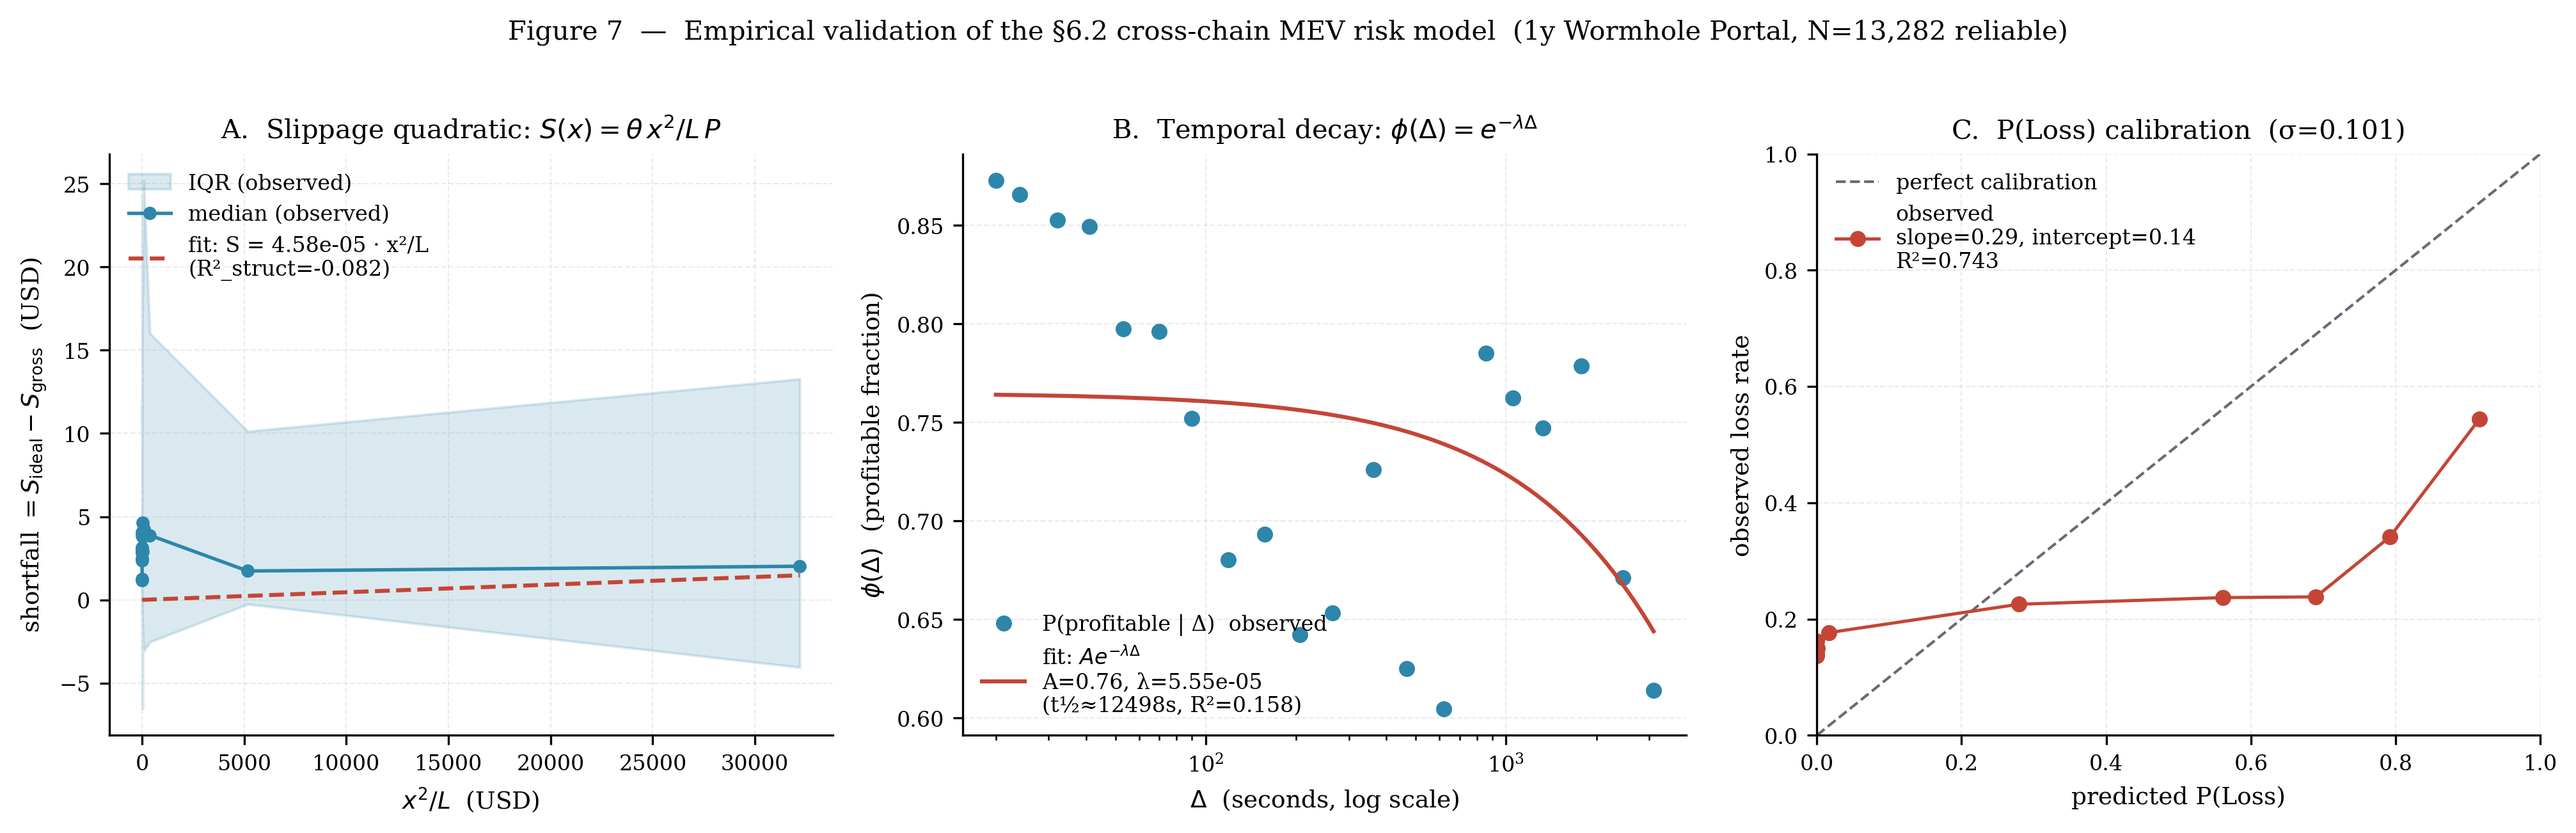
\includegraphics[width=0.99\textwidth]{07_risk_validation.png}
    \caption{Direct tests of the baseline risk model
    (Section~\ref{sec:ch4-refined-model}): (a) quadratic-slippage test;
    (b) pure-exponential $\phi$ test; (c) log-normal $P(\text{Loss})$
    decile calibration with pooled $\sigma$.}
    \label{fig:ch4-validation}
\end{figure*}

\paragraph{Walk-through of Figure~\ref{fig:ch4-validation}.}
Panel~A scatters observed shortfall
($S_{\text{ideal}} - S_{\text{gross}}$) against the baseline
predictor $x^{2}/L$ with the fitted line overlaid: the cloud shows
very weak linear structure and the structural
$R^{2}_{\text{struct}}$ is $-0.08$, i.e.\ the model fits worse than
a flat intercept, visually disproving the quadratic form in the
observed \$10--\$10\,k size range. Panel~B overlays a
pure-exponential $A\,e^{-\lambda\Delta}$ onto the empirical
$\phi(\Delta)$ curve on a log-$\Delta$ axis; the overlay
systematically undershoots at long $\Delta$ because it cannot
capture the clearly non-zero asymptote near $70\%$, yielding a
modest fit $R^{2}\!=\!0.16$. Panel~C is a 10-decile calibration of
predicted $P(\text{Loss})$ (built from the pooled $\sigma\!=\!0.101$)
against observed loss rate; the points systematically lie above the
$45^{\circ}$ line at high deciles, i.e.\ the baseline
\emph{over-predicts} tail loss probability, yielding calibration
$R^{2}\!=\!0.741$ but with an inflated slope of $0.286$.

\clearpage
\begin{figure*}[!t]
    \centering
    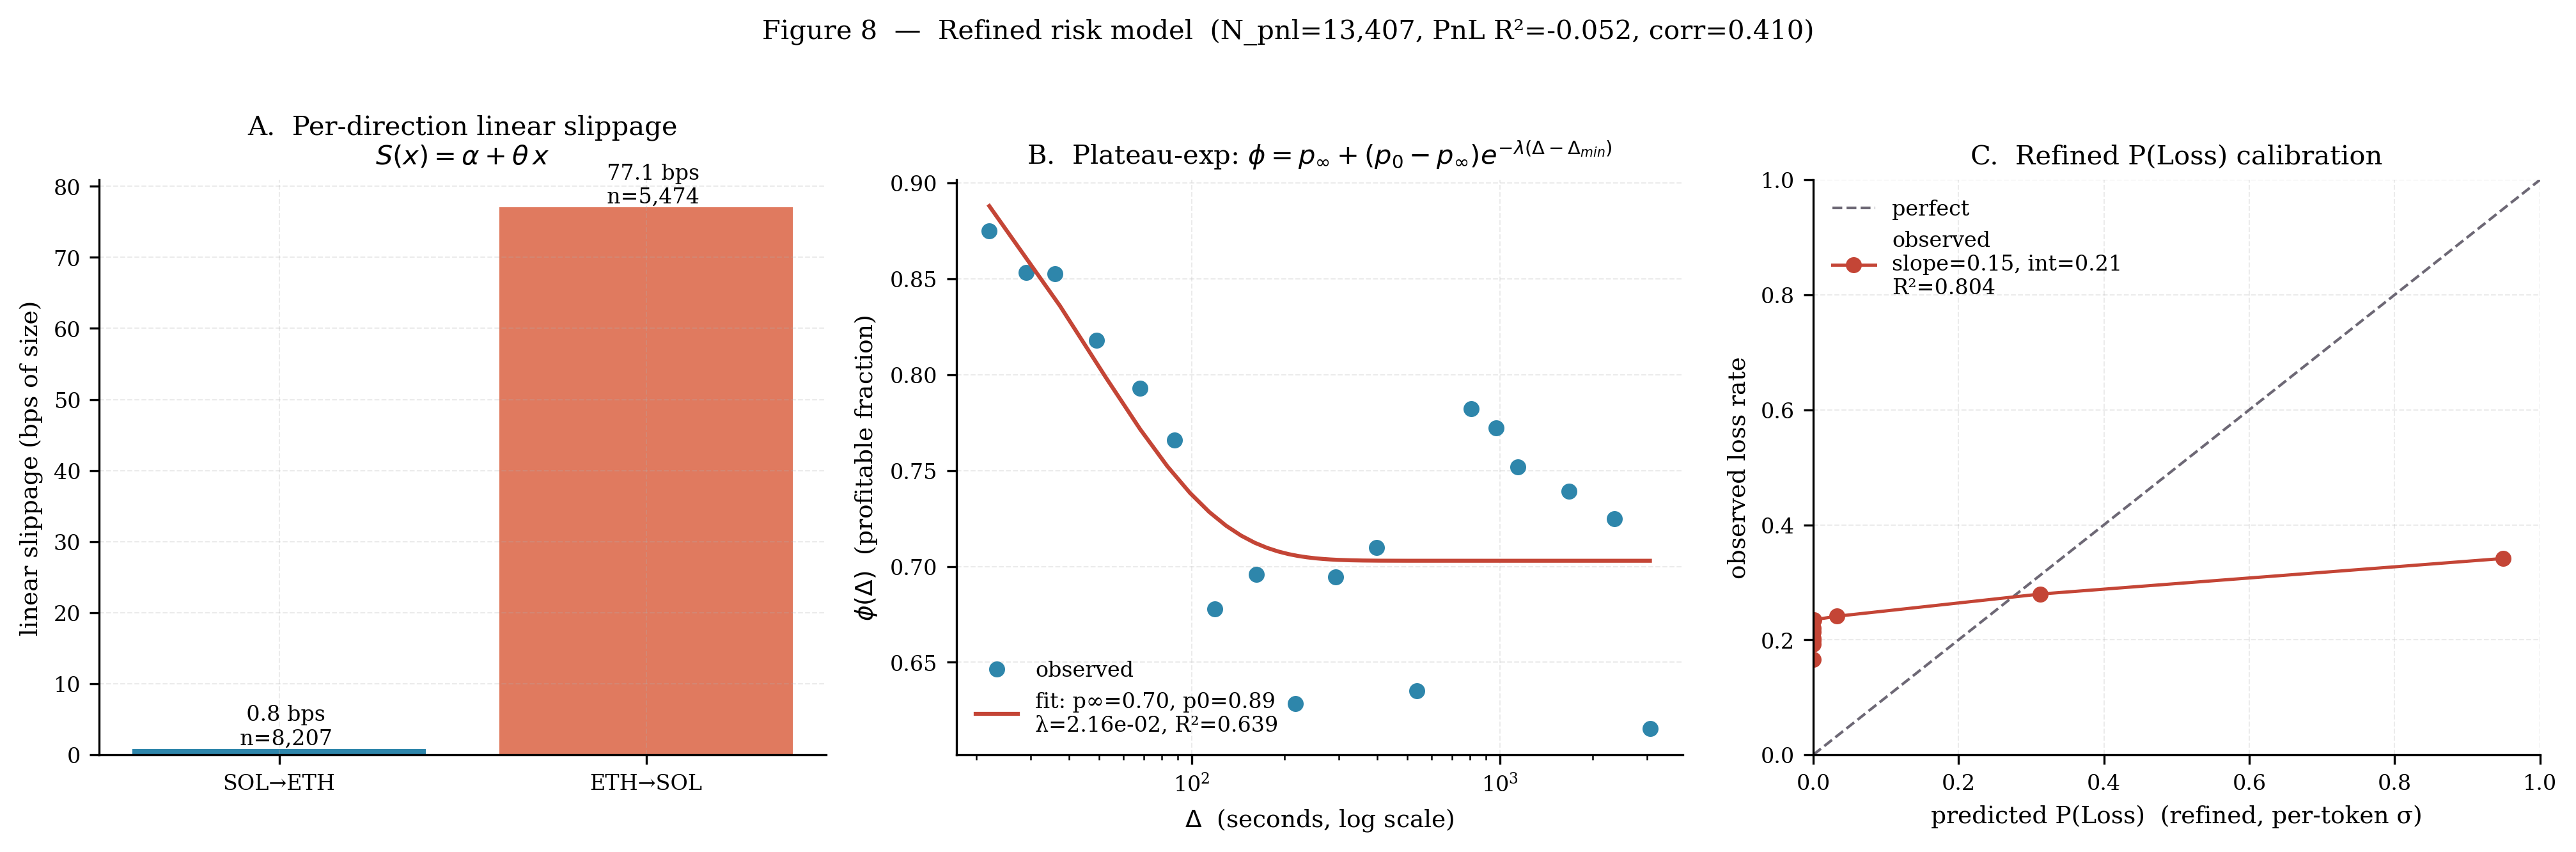
\includegraphics[width=0.99\textwidth]{08_refined_validation.png}
    \caption{Same tests, under the refined model: (a) direction-specific
    linear slippage bars; (b) plateau-exp $\phi$ fit; (c) $P(\text{Loss})$
    calibration with per-token $\hat\sigma_{\text{tok}}$.}
    \label{fig:ch4-validation2}
\end{figure*}

\paragraph{Walk-through of Figure~\ref{fig:ch4-validation2}.}
Panel~A replaces the pooled scatter with two per-direction bars of
the fitted slope $\hat\theta$ in bps-of-size: \SolEth{} at $0.84$~bps
is essentially flat, while \EthSol{} at $77$~bps is two orders of
magnitude larger --- an asymmetry that was completely invisible
under the pooled baseline form. Panel~B overlays the plateau-exp fit
$\phi(\Delta) = p_{\infty} + (p_{0}-p_{\infty})\,e^{-\lambda(\Delta-\Delta_{\min})}$
onto the same $\phi(\Delta)$ data: the fitted curve now hits both
the early exponential decay and the long-latency plateau at
$p_{\infty}\!=\!0.703$, with fit $R^{2}$ jumping from $0.16$ to
$\mathbf{0.638}$. Panel~C redoes the decile calibration of
$P(\text{Loss})$ using the per-token estimator
$\hat\sigma_{\text{tok}}$ (median $0.040$): the decile dots now lie
much closer to the $45^{\circ}$ line ($R^{2}\!=\!\mathbf{0.806}$),
and the regression slope collapses from $0.286$ to $0.149$. The
refined model now mildly \emph{under}-predicts absolute loss rate,
but the rank order of deciles remains essentially monotone --- which
is exactly what the binary admit/reject decision rule of
Eq.~\eqref{eq:ch4-decision} requires.

\begin{table*}[t]
    \centering
    \small
    \caption{Parameter estimates --- baseline vs.\ refined risk model.}
    \label{tab:ch4-validation}
    \begin{tabular}{lcc}
        \toprule
        & Baseline (§4.3.1) & Refined (§4.3.2) \\
        \midrule
        Slippage form & $\theta\,x^{2}/L$ & dir-specific $\alpha + \theta\,x$ \\
        $\;\hat\theta$ & $4.6\!\times\!10^{-5}$ & \SolEth:\,$0.84$\,bps; \EthSol:\,$77.1$\,bps \\
        $\;R^{2}_{\text{struct}}$ & $-0.08$ & $0.00025$ / $0.113$ \\
        \addlinespace
        $\phi(\Delta)$ form & $A\,e^{-\lambda\Delta}$ & $p_{\infty}+(p_{0}-p_{\infty})e^{-\lambda(\Delta-\Delta_{\min})}$ \\
        $\;$fit $R^{2}$ & $0.16$ & $\mathbf{0.638}$ \\
        $\;\hat\lambda$ & $5.6\!\times\!10^{-5}$ s$^{-1}$ & $2.16\!\times\!10^{-2}$ s$^{-1}$ \\
        $\;\hat p_{\infty}$ & --- & $0.703$ \\
        $\;\hat p_{0}$ & --- & $0.888$ \\
        \addlinespace
        $\sigma$ used for $P(\text{Loss})$ & pooled: $0.101$ & per-token median: $0.040$ \\
        Calibration $R^{2}$ & $0.741$ & $\mathbf{0.806}$ \\
        Calibration slope & $0.286$ & $0.149$ \\
        Calibration intercept & $0.142$ & $0.210$ \\
        \bottomrule
    \end{tabular}
\end{table*}

\subsection{Parameter Estimates}

Table~\ref{tab:ch4-validation} reports parameter estimates and fit
diagnostics for both models.

\paragraph{Slippage.} The refined, direction-specific linear form reveals
a striking asymmetry: \SolEth{} effective slippage is $\approx\!0.84$~bps
per unit size (essentially zero), while \EthSol{} is $\approx\!77$~bps ---
two orders of magnitude larger, with a vastly better structural fit
($R^{2}\!=\!0.113$ vs.\ $0.00025$). This confirms that the bulk of the
slippage cost lives in the \EthSol{} direction, which has the long
latency, larger gaps, and more concentrated memecoin exposure.

\paragraph{Temporal decay.} The plateau-exp form lifts the fit from
$R^{2}\!=\!0.16$ to $R^{2}\!=\!0.638$, a near-fourfold improvement. The
estimated floor $p_{\infty}\!=\!0.703$ quantifies the ``residual''
profitability that the pure-exp form was unable to explain: even for
latencies up to $1$~hour, $\approx\!70\%$ of arbitrage events remain
profitable, which is consistent with the bimodal speed profile observed
in Figure~\ref{fig:ch4-timing}.

\paragraph{Loss probability.} The refined $P(\text{Loss})$ calibration
$R^{2}$ improves from $0.741$ to $\mathbf{0.806}$. The compressed slope
($0.149$) indicates that even with $\hat\sigma_{\text{tok}}$ the absolute
scale is still miscalibrated (the model now \emph{under}-predicts rather
than over-predicts), but the \emph{rank order} remains strong --- the
decile with the highest predicted $P(\text{Loss})$ is always the decile
with the highest observed loss rate. In practice this is exactly what is
needed for Eq.~\eqref{eq:ch4-decision}: a monotone classifier of risk.

\subsection{PnL Prediction via the Combined Refined Model}

We finally evaluate the closed-form predictor $\widehat{\Pi}_{\text{net}}$
from Eq.~\eqref{eq:ch4-pi-hat} against observed net PnL on the
$N=13{,}682$ reliable subset with resolved entry gap. Restricted to the
middle-98\% band of both observed and predicted PnL, the
Pearson correlation is $\rho\!=\!0.410$ while the structural
$R^{2}$ is weakly negative ($-0.052$).

This result has a clean interpretation. The closed-form predictor carries
non-trivial signal about direction and magnitude (confirmed by
$\rho\!=\!0.41$) but cannot explain idiosyncratic per-token behaviour
(evident in $R^{2}<0$). The discrepancy quantifies exactly what the
machine-learning model of Section~\ref{sec:ch4-empirical} recovers through
$\texttt{exit\_coverage}$ and token-specific interactions: features that
the analytical model cannot embed without per-token parameter estimation.
In other words, \textbf{the refined analytical model is a sound
\emph{risk-judgement} tool but not, by itself, a \emph{PnL-forecasting}
tool}. Its operational role is Eq.~\eqref{eq:ch4-decision} --- binary
admit/reject --- while quantitative PnL estimation is best delegated to
the data-driven model of Figure~\ref{fig:ch4-model}.

\subsection{Summary Judgement Matrix}

Table~\ref{tab:ch4-summary} summarises the empirical answer to the
original theoretical claims.

\begin{table*}[t]
    \centering
    \small
    \caption{Empirical verdict on each theoretical prediction.}
    \label{tab:ch4-summary}
    \begin{tabular}{lcccc}
        \toprule
        Prediction & Sign & Rank & Functional form & Refinement \\
        \midrule
        Latency asymmetry $\Delta_{\mathrm{E}\to\mathrm{S}}\!\gg\!\Delta_{\mathrm{S}\to\mathrm{E}}$ & \checkmark & \checkmark & n/a & --- \\
        Slippage grows in $x$ & \checkmark & \checkmark & linear, not quadratic & R1 \\
        $\phi(\Delta)$ decays in $\Delta$ & \checkmark & \checkmark & plateau-exp, not pure exp & R2 \\
        $P(\text{Loss})$ monotone in $\Delta,\Cexec/\Rgross$ & \checkmark & \checkmark & pooled $\sigma$ over-predicts & R3 \\
        Combined $\widehat{\Pi}_{\text{net}}$ usable for entry/exit decision & \checkmark & \checkmark & R1+R2+R3 composite & --- \\
        Combined $\widehat{\Pi}_{\text{net}}$ as PnL forecast & --- & --- & --- & delegate to ML \\
        \bottomrule
    \end{tabular}
\end{table*}

The refined model is a \textbf{risk-judgement} tool whose \textbf{rank
fidelity} is strong enough to support the binary admit/reject decision
rule of Eq.~\eqref{eq:ch4-decision}. Quantitative PnL estimation is ceded
to the data-driven gradient-boosting model, whose $R^{2}_{\text{CV}}\!=\!0.789$
benchmark was reported in Section~\ref{sec:ch4-empirical}. Together these
two models form the two halves of the complete Wormhole cross-chain MEV
decision stack: \emph{analytical} for admit/reject, \emph{data-driven} for
sizing and timing.

\end{document}
